\documentclass[16pt,a4paper]{article}

%%%%%%%%%%%%%%%%%%%%%%%%%%%%%%% PACKAGES %%%%%%%%%%%%%%%%%%%%%%%%%%%%%%%%
\usepackage{tikz}
\usetikzlibrary{decorations.pathmorphing}
\usepackage{amsmath}
\usepackage{float}
\usepackage{framed}  % For boxing the figure

\usepackage{geometry}
 \geometry{
 a4paper,
 total={170mm,257mm},
 left=20mm,
 top=20mm,
 }
\usepackage{graphicx}
\usepackage{wrapfig}
\usepackage{float}
\graphicspath{ {./images/} }

\usepackage{courier}
\renewcommand*\familydefault{\ttdefault} 
\usepackage[T1]{fontenc}

\usepackage[english]{babel}
\pagenumbering{arabic}
\usepackage{ae,aecompl}
\usepackage{fancyhdr}

\pagestyle{fancy}
\fancyhf{}
\lhead{Coupled Oscillator}
\rfoot{Page \thepage}


\begin{document}
\title{Understanding Coupled Oscillators}
\author{Suhas P K}
\date{\today}


\maketitle

\section{Introduction}


\begin{figure}[H]
    \centering
    \fbox{  % Start the box around the figure
    \begin{minipage}{\linewidth}  % Create a minipage to contain the diagram and caption
        \centering
        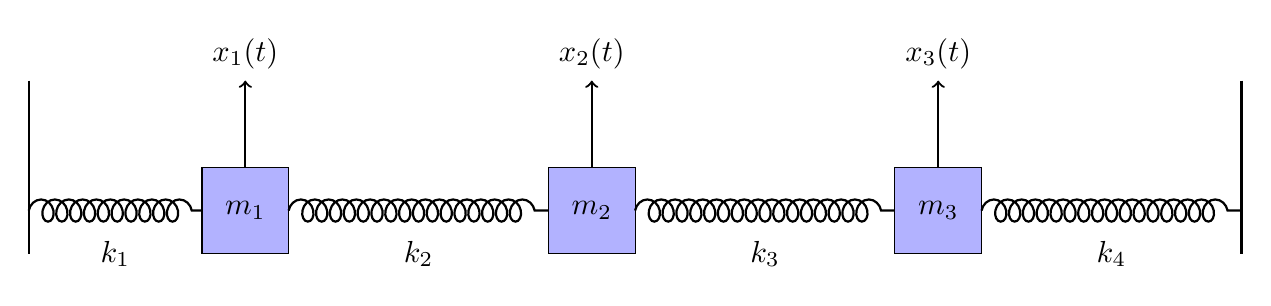
\begin{tikzpicture}[scale=1.1, every node/.style={scale=1.1}]
            % Draw fixed walls
            \draw[thick] (0,0.5) -- (0,-1.5);
            \draw[thick] (14,0.5) -- (14,-1.5);
            
            % Draw the masses
            \draw[fill=blue!30] (2,-0.5) rectangle (3,-1.5) node[pos=.5] {$m_1$};
            \draw[fill=blue!30] (6,-0.5) rectangle (7,-1.5) node[pos=.5] {$m_2$};
            \draw[fill=blue!30] (10,-0.5) rectangle (11,-1.5) node[pos=.5] {$m_3$};
            
            % Draw the springs, attached to the walls and between the masses
            \draw[thick,decorate,decoration={coil,aspect=0.8,amplitude=4pt,segment length=5pt}] (0,-1) -- (2,-1);    % Spring k1
            \draw[thick,decorate,decoration={coil,aspect=0.8,amplitude=4pt,segment length=5pt}] (3,-1) -- (6,-1);    % Spring k2
            \draw[thick,decorate,decoration={coil,aspect=0.8,amplitude=4pt,segment length=5pt}] (7,-1) -- (10,-1);   % Spring k3
            \draw[thick,decorate,decoration={coil,aspect=0.8,amplitude=4pt,segment length=5pt}] (11,-1) -- (14,-1);  % Spring k4
            
            % Labels for springs
            \node at (1,-1.5) {$k_1$};
            \node at (4.5,-1.5) {$k_2$};
            \node at (8.5,-1.5) {$k_3$};
            \node at (12.5,-1.5) {$k_4$};
            
            % Displacement markers
            \draw[->,thick] (2.5,-0.5) -- (2.5,0.5) node[above] {$x_1(t)$};
            \draw[->,thick] (6.5,-0.5) -- (6.5,0.5) node[above] {$x_2(t)$};
            \draw[->,thick] (10.5,-0.5) -- (10.5,0.5) node[above] {$x_3(t)$};
            
            % Ground for fixed walls
            \draw[thick] (0,-1) -- (0,-1.2);
            \draw[thick] (14,-1) -- (14,-1.2);
            
        \end{tikzpicture}
        \caption{A diagram representing a coupled oscillator system with three masses \( m_1, m_2, m_3 \) connected by springs \( k_1, k_2, k_3, k_4 \). The masses are displaced by distances \( x_1(t), x_2(t), x_3(t) \) over time.}
        \label{fig:coupled_oscillator}
    \end{minipage}
    }  % End the box
\end{figure}




In this document, we will derive the equations of motion for a coupled harmonic oscillator system and apply them to a real-world example of a \textbf{CO\textsubscript{2} molecule}. The CO\textsubscript{2} molecule can be modeled as three masses (the oxygen and carbon atoms) connected by springs (representing the molecular bonds). This model provides insights into how the vibrational modes of the molecule can be understood using the principles of coupled oscillators.

We will use \textbf{Bloom’s Taxonomy} to progressively build our understanding of this system, from basic recall to advanced problem-solving. 

\section{Remembering (Knowledge)}
\subsection{Basic Definition}
A \textbf{coupled harmonic oscillator} is a system of two or more masses connected by springs such that the motion of one mass affects the others. In general, these systems can be described by the following equation:
\begin{equation}
m_i \ddot{x}_i = -k(x_i - x_{i-1}) - k(x_i - x_{i+1}),
\end{equation}
where $x_i$ is the displacement of the $i$-th mass, $k$ is the spring constant, and $m_i$ is the mass.

\section{Understanding (Comprehension)}
In a coupled oscillator system, the behavior of each oscillator depends on its neighbors. Consider the linear chain of masses and springs for the CO\textsubscript{2} molecule:
\begin{itemize}
    \item Each oxygen atom is modeled as a mass, and the carbon atom is also a mass.
    \item The bonds between the atoms are modeled as springs.
\end{itemize}

Example:
In CO\textsubscript{2}, we have:
\begin{itemize}
    \item Masses: Carbon ($C$) and two Oxygen atoms ($O$).
    \item Springs: Molecular bonds between the atoms, modeled as spring constants $k$.
\end{itemize}

\section{Applying (Application)}
To derive the equations of motion for this system, we consider the following:
\begin{align}
m \ddot{x}_1 &= -k(x_1 - x_2), \tag{2} \\
m \ddot{x}_2 &= -k(x_2 - x_1) - k(x_2 - x_3), \tag{3} \\
m \ddot{x}_3 &= -k(x_3 - x_2). \tag{4}
\end{align}
These equations describe the forces on each mass due to its neighboring masses. 

\textbf{Eigenvalue Problem:}
To solve this system, we express it in matrix form:
\begin{equation}
m \ddot{\mathbf{x}} = -k \mathbf{A} \mathbf{x}, \tag{5}
\end{equation}
where $\mathbf{x}$ is the vector of displacements and $\mathbf{A}$ is the coupling matrix:
\begin{equation}
\mathbf{A} = \begin{pmatrix}
  2 & -1 & 0 \\
  -1 & 2 & -1 \\
  0 & -1 & 2
\end{pmatrix}. \tag{6}
\end{equation}

\section{Analyzing (Analysis)}
The system of equations can be analyzed using normal modes. We seek solutions of the form $x_i(t) = X_i \cos(\omega t + \phi)$, where $\omega$ is the angular frequency. Substituting this into the matrix equation yields the eigenvalue problem:
\begin{equation}
\mathbf{A} \mathbf{X} = \lambda \mathbf{X}, \tag{7}
\end{equation}
where $\lambda = \frac{\omega^2}{k/m}$ are the eigenvalues, and $\mathbf{X}$ are the eigenvectors corresponding to the normal modes of the system.

Interpretation for CO\textsubscript{2}:
The eigenvalues represent the frequencies of the vibrational modes of the CO\textsubscript{2} molecule, and the eigenvectors describe the relative motion of the atoms during these vibrations.

\section{Evaluating (Evaluation)}
To evaluate this system, we can compute the normal mode frequencies for the CO\textsubscript{2} molecule and compare them to experimental data. For the CO\textsubscript{2} molecule, the three normal modes are:
\begin{itemize}
    \item Symmetric stretching
    \item Asymmetric stretching
    \item Bending mode
\end{itemize}

These modes correspond to different ways in which the atoms can vibrate relative to each other. By solving the eigenvalue problem, we can find the corresponding frequencies for each mode.

\section{Creating (Synthesis)}
Finally, we can extend this analysis to more complex molecules. For example, we could model a molecule like methane (CH\textsubscript{4}), where there are more atoms and more complex vibrational modes. By applying the same principles, we can analyze the normal modes of any molecule, giving us a powerful tool for understanding molecular vibrations in physics and chemistry.

\section{Conclusion}
In this document, we have derived the equations of motion for a coupled harmonic oscillator system and applied them to a real-world example of a CO\textsubscript{2} molecule. Using Bloom’s Taxonomy, we have progressively built up our understanding of the system, from basic knowledge to advanced analysis and synthesis. Coupled harmonic oscillators are a fundamental concept in many areas of physics and have important applications in molecular physics, electrical engineering, and beyond.



\end{document}
